\let\negmedspace\undefined
\let\negthickspace\undefined
\documentclass[journal]{IEEEtran}
\usepackage[a5paper, margin=10mm, onecolumn]{geometry}
%\usepackage{lmodern} % Ensure lmodern is loaded for pdflatex
\usepackage{tfrupee} % Include tfrupee package

\setlength{\headheight}{1cm} % Set the height of the header box
\setlength{\headsep}{0mm}     % Set the distance between the header box and the top of the text

\usepackage{gvv-book}
\usepackage{comment}
\usepackage{gvv}
\usepackage{cite}
\usepackage{amsmath,amssymb,amsfonts,amsthm}
\usepackage{algorithmic}
\usepackage{graphicx}
\usepackage{textcomp}
\usepackage{xcolor}
%\usepackage{txfonts}
\usepackage{listings}
\usepackage{enumitem}
\usepackage{mathtools}
\usepackage{gensymb}
\usepackage{comment}
\usepackage[breaklinks=true]{hyperref}
\usepackage{tkz-euclide} 
\usepackage{listings}
% \usepackage{gvv}                                        
\def\inputGnumericTable{}                                 
\usepackage[latin1]{inputenc}                                
\usepackage{color}                                            
\usepackage{array}                                            
\usepackage{longtable}                                       
\usepackage{calc}                                             
\usepackage{multirow}                                         
\usepackage{hhline}                                           
\usepackage{ifthen}                                           
\usepackage{lscape}
\usepackage{circuitikz}
\tikzstyle{block} = [rectangle, draw, fill=blue!20, 
    text width=4em, text centered, rounded corners, minimum height=3em]
\tikzstyle{sum} = [draw, fill=blue!10, circle, minimum size=1cm, node distance=1.5cm]
\tikzstyle{input} = [coordinate]
\tikzstyle{output} = [coordinate]


\begin{document}

\bibliographystyle{IEEEtran}
\vspace{3cm}

\title{9.4.18}
\author{EE25BTECH11006 - ADUDOTLA SRIVIDYA}
\maketitle
    {\let\newpage\relax\maketitle}

\renewcommand{\thefigure}{\theenumi}
\renewcommand{\thetable}{\theenumi}
\setlength{\intextsep}{10pt} % Space between text and floats

\numberwithin{equation}{enumi}
\numberwithin{figure}{enumi}
\renewcommand{\thetable}{\theenumi}

\textbf{Question}: \\
Find the roots of the quadratic equation graphically.
\begin{align}
4x^2 + 4\sqrt{3}x + 3 = 0
\end{align}

\solution \\

\begin{align}
y = 4x^2 + 4\sqrt{3}x + 3
\end{align}

This equation can be represented as the conic:
\begin{align}
\vec{x}^T\vec{V}\vec{x} + 2\vec{u}^T\vec{x} + f = 0
\end{align}
where
\begin{align}
\vec{V} = \myvec{4 & 0 \\ 0 & 0}, \quad \vec{u} = \myvec{2\sqrt{3} \\ 0}, \quad f = 3
\end{align}

To find the roots, we find the points of intersection of the conic with the x-axis:
\begin{align}
\vec{x} = \vec{h} + k_i\vec{m}    
\end{align}
\begin{align}
\vec{h}=\myvec{0 \\ 0}, \quad \vec{m} = \myvec{1 \\ 0}
\end{align}

Substitute into the conic equation:
\begin{align}
(\vec{h} + k_i \vec{m})^{\top} \vec{V} (\vec{h} + k_i \vec{m}) + 2\vec{u}^{\top} (\vec{h} + k_i \vec{m}) + f = 0
\end{align}

This simplifies to a quadratic in \( k_i \):
\begin{align}
k_i^2 \vec{m}^T \vec{V} \vec{m} + 2k_i \vec{m}^T (\vec{V}\vec{h} + \vec{u}) + g(\vec{h}) = 0
\end{align}

Now substituting the values:
\begin{align}
k_i = \frac{ -\vec{m}^T(\vec{V}\vec{h} + \vec{u}) \pm \sqrt{ [\vec{m}^T(\vec{V}\vec{h} + \vec{u})]^2 - \vec{m}^T\vec{V}\vec{m} \cdot g(\vec{h}) } }{\vec{m}^T \vec{V} \vec{m}}
\end{align}

\begin{align}
\Rightarrow k_i = \frac{ -2\sqrt{3} \pm \sqrt{ (2\sqrt{3})^2 - 4 \cdot 4 \cdot 3 } }{4}
= \frac{ -2\sqrt{3} \pm \sqrt{12 - 12} }{4}
= \frac{ -2\sqrt{3} }{4}
= \frac{-\sqrt{3}}{2}
\end{align}

Hence, the only real root is:
\begin{align}
\vec{x} = \vec{h} + k_i\vec{m} = \myvec{-\frac{\sqrt{3}}{2} \\ 0}
\end{align}

\begin{figure}[h!]
    \centering
    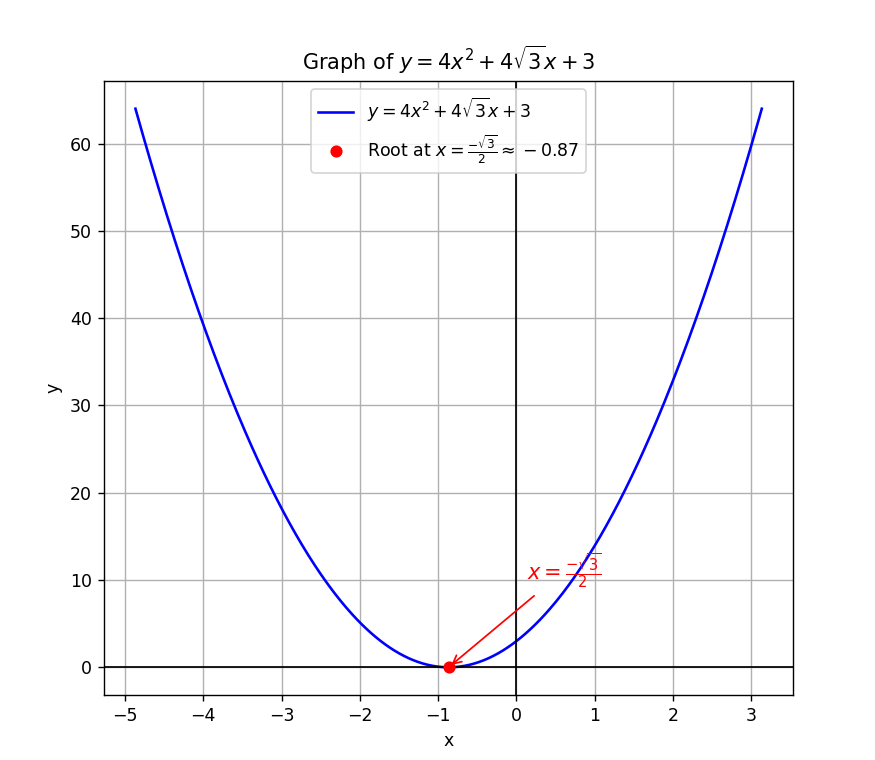
\includegraphics[height=0.5\textheight]{figs/fig.png}
    \caption{Graph of \( y = 4x^2 + 4\sqrt{3}x + 3 \) showing a double root}
    \label{figure_9_4_184}
\end{figure}

\end{document}
